%%%%%%%%%%%%%%%%%%%%%%%%%%%%%%%%%%%%%%%%%%%%%%%%%%%%%%%%%%%%%%%%%%%%%%%%
%                                                                      %
%     File: Proposed_control.tex                                  	   %
%     Tex Master: Thesis.tex                                           %
%                                                                      %
%     Author: Israel Sother                                            %
%     Last modified: 27 May 2024                                       %
%                                                                      %
%%%%%%%%%%%%%%%%%%%%%%%%%%%%%%%%%%%%%%%%%%%%%%%%%%%%%%%%%%%%%%%%%%%%%%%%
\section{Control Methods Development}
\label{section:Control Methods Development}%chktex 24

In this section some of the main \glspl{mpc} used on the power converters field are developed. At the end of the section, the proposed control strategy is presented. The methods compared with the manufacturer's \gls{foc} are:
\begin{itemize}
	\item Finite Set \gls{mpc}
	\item Finite Set with null vector \gls{mpc}
	\item Non-Linear Continuous Set \gls{mpc}
	\item \acrfull{rush}
\end{itemize}
All those methods rely on the line current and rotor position encoder data to estimate the currents in the dq0 frame. The DC Link voltage is also measured to account for battery voltage fluctuation. The control strategy is then applied to the motor model to predict the next time step values. This processed data is refreshed at each time step to be utilized by the selected control strategy.
Although it is possible to use multiple horizon prediction steps, to keep the computational cost low, and maintain high switching frequencies, all the proposed methods use a horizon of only 1 discretized time step. 
% This is later verified as not having an expressive take on performance as the system is fast enough so that the dynamics are well represented with only one timestep.

Some of these control methods depend on a cost function definition to choose the best control action. The control action that minimizes this cost function is then applied to the system.
\begin {subequations}
	\begin{equation}
	\begin{aligned}
		\mathcal{J} =  s_1 \left(\frac{i_{d_{ref}}-i_{d_{k+1}}}{i_{d_{ref}}}\right)^2 + s_2 \left(\frac{i_{q_{ref}}-i_{q_{k+1}}}{i_{q_{ref}}}\right)^2 + \mathcal{C}_{soft}
	\end{aligned}
	\label{eq:cost_mpc}
	\end{equation}
	\begin{equation}
	\mathcal{C}_{soft} = s_3 \max\left(0,\sqrt{i_{d_{k+1}}^2 + i_{q_{k+1}}^2} - \sqrt{\frac{2}{3}} i_{line max}\right) + s_4 \max\left(0,\sqrt{u_{d_{k+1}}^2+u_{q_{k+1}}^2}-V_{DC}\right)
	\label{eq:soft_constraints_mpc}
	\end{equation}
\end{subequations}
The cost function shown in \Cref{eq:cost_mpc} is composed of the error between the reference and the predicted values of the currents, and a soft constraint that penalizes the system for exceeding the maximum line current or the DC link voltage while some gains $s_x$ are used to adjust the priorities. The soft constraint is defined in \Cref{eq:soft_constraints_mpc}.

\subsection{Finite Set MPC}
In a \gls{fsmpc} each of the basic vectors defined on \Cref{table:space_vector} are applied to \Cref{eq:motor_backward_euler_matrix} using the current measured data, resulting in different predictions for the next time step values. A cost function that compares the torque and currents (to account for \gls{mtpa}) with the references, is then evaluated for each of those predictions. The vector with the lowest cost is then applied at the next time step, as shown in \Cref{fig:FSMPC_Diagram}.
\begin{figure}[!htb]
	\centering
	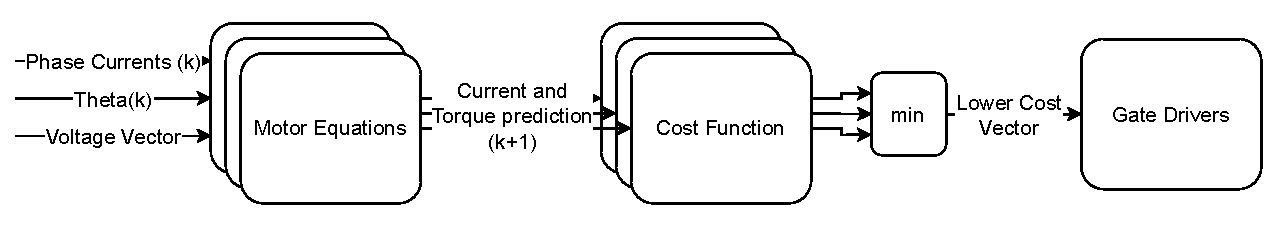
\includegraphics[width=0.8\textwidth]{Figures/FSMPC.pdf}
	\caption[FSMPC Diagram.]{FSMPC Diagram.}
	\label{fig:FSMPC_Diagram}%chktex 24
\end{figure}

\subsection{Finite Set with Null Vector MPC}

Although effective, the simple Finite Set \gls{mpc} can incur heavy torque ripple, due to its limited options on which vector can be applied. That behavior can be exacerbated by low power operation points, where the active vectors result in a bigger percentual change in currents. This problem can be mitigated by introducing the possibility of sharing the sample time between the chosen active vector and a null vector. Such an approach allows the control to apply vectors that point in the direction of the native ones but have smaller amplitude.

This addition of a null vector comes with the problem of now having virtually infinite vector options (depending on the \gls{pwm} resolution), but that can be solved with some approximations. This method begins as the previous one, where each of the 7 possible vectors is applied to the motor model, but before passing those results for the cost function the predicted torque is compared with the reference. If a crossing is detected, meaning the values $T_{ref} - T_{e(k)}$ and $T_{ref} - T_{e(k+1)}$ have different signals the algorithm assumes that the ideal vector has a smaller amplitude, thus computes a ratio of active vector time and null vector time. To calculate such a ratio an approximation was made that, given the short sample time, the complete system is assumed to behave linearly during that period. If the system behaves linearly, the currents and torque for a combination of null and active vectors will also be a linear combination of the individual values for each vector multiplied by its application time. This approximation is shown in \Cref{eq:linear_combination,eq:linear_combination_torque}, where $d$ is the duty cycle value for a given vector, and the subscripts $_{act}$ and $_n$ represents the active and null vectors respectively.

\begin{equation}
	i_x = i_{act} d_{act} + i_n d_n
	\label{eq:linear_combination}
\end{equation}
\begin{equation}
	T_x = T_{act} d_{act} + T_n d_n = T_{act} d_{act} + T_n - T_n d_{act}
	\label{eq:linear_combination_torque}
\end{equation}

With that property, and knowing that $d_{act} + d_n = 1$ the duty cycle for the active vector is calculated as shown in \Cref{eq:duty_cycle}.

\begin{equation}
	d_{act} = \frac{T_{ref} - T_n}{T_{act}-T_n}
	\label{eq:duty_cycle}
\end{equation}


Given the duty cycle, the predictions are updated and passed to the cost function, which chooses the best combination of active and null vectors. A diagram of this method is shown in \Cref{fig:FSMPC_null_Diagram}.

\begin{figure}[!htb]
	\centering
	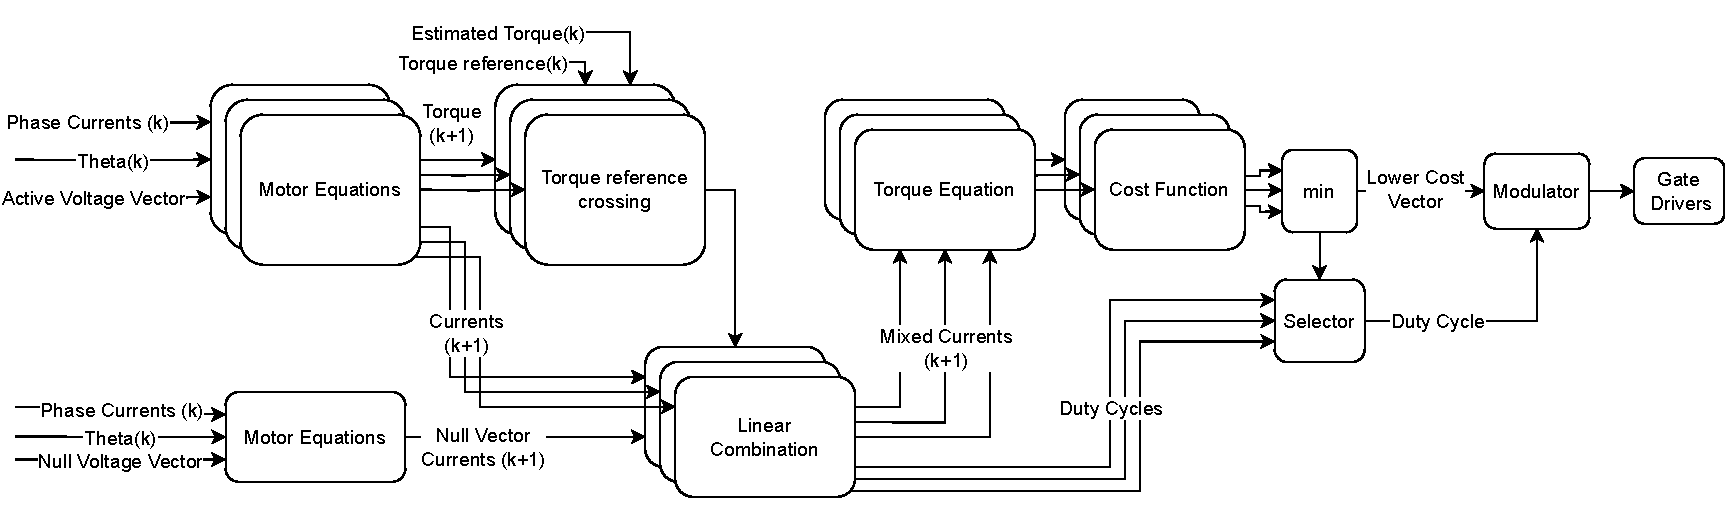
\includegraphics[width=1\textwidth]{Figures/FSMPC_null_vector.pdf}
	\caption[Finite Set with Null Vector MPC Diagram.]{Finite Set with Null Vector MPC Diagram.}
	\label{fig:FSMPC_null_Diagram}%chktex 24
\end{figure}

\subsection{Non-Linear Continuous Set MPC}

In the continuous set \glspl{mpc} the control action is not limited to a finite set of vectors, but it is assumed that any vector attainable by a defined modulation technique is available. This increases the complexity of the control, as the control action locus becomes infinite.
 This approach is very similar to the most common approach of \gls{mpc} used in other fields that are not power systems. It takes an implicit approach, where the motor model shown in \Cref{eq:motor_backward_euler_matrix} is combined with an optimization solver that numerically finds the best control action. This \gls{mpc} technique has the advantage of easy constraints implementation while having the benefits of a continuous set controller. This advantage comes at the cost of largely increased computational time, as it needs to evaluate the model equation several times to find the optimal voltage vector that fulfills the constraints. This additional complexity can often be prohibitive for power systems where a fast-acting control is needed. The diagram of this method is shown in \Cref{fig:implicit_csmpc_diagram}.

\begin{figure}[!htb]
	\centering
	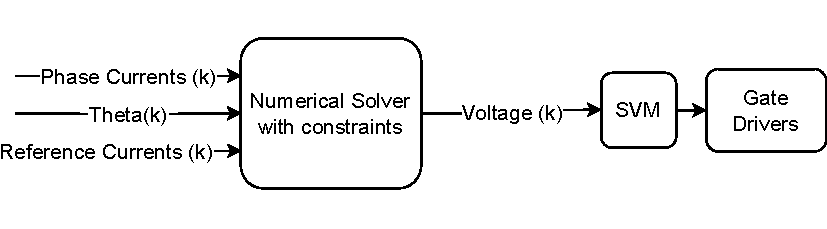
\includegraphics[width=0.65\textwidth]{Figures/Implicit_CSMPC.pdf}
	\caption[Implicit Continuous Set MPC Diagram.]{Implicit Continuous Set MPC Diagram.}
	\label{fig:implicit_csmpc_diagram}%chktex 24
\end{figure}

\subsection{RUSH MPC}

One of the advantages of the approximations made in the discretization process is that even though the matrices change in time, for a given moment the system is linear, and as such an inverse dynamic can be derived. So, if in \Cref{eq:motor_backward_euler_matrix} the currents on the next step are replaced by a reference for the current vector, the necessary applied voltage can be calculated in real-time. This is done by \Cref{eq:Vdq}.

\begin{equation}
	\begin{aligned}
		\begin{bmatrix}
			u_{d(k+1)} \\
			u_{q(k+1)} \\
		\end{bmatrix}
		=
		\begin{bmatrix}
			\frac{h}{hr+L_{d(i_d(k))}} & 0                          \\
			0                          & \frac{h}{hr+L_{q(i_q(k))}} \\
		\end{bmatrix}^{-1} \\
		\left(
		\begin{bmatrix}
				1                                                    & -h\frac{\omega_{e(k)}L_{q(i_q(k))}}{hr+L_{d(i_d(k))}} \\
				h\frac{\omega_{e(k)}L_{d(i_d(k))}}{hr+L_{q(i_q(k))}} & 1                                                     \\
			\end{bmatrix}
		\begin{bmatrix}
				i_{d_{ref}} \\
				i_{q_{ref}} \\
			\end{bmatrix}
		-
		\begin{bmatrix}
				\frac{L_{d(i_d(k))}}{hr+L_{d(i_d(k))}} & 0                                      \\
				0                                      & \frac{L_{q(i_q(k))}}{hr+L_{q(i_q(k))}} \\
			\end{bmatrix}
		\begin{bmatrix}
				i_{d(k)} \\
				i_{q(k)} \\
			\end{bmatrix}
		-
		\begin{bmatrix}
				0                                                 \\
				-h\frac{\omega_{e(k)}\psi_{PM}}{hr+L_{q(i_q(k))}} \\
			\end{bmatrix}
		\right)
	\end{aligned}
	\label{eq:Vdq}
\end{equation}

This approach is commonly used in linear unconstrained \glspl{mpc} to improve computation times, where a control law is precomputed and stored in memory. But in the presented case there is an important constraint that is not accounted for in the previous equation. When very short time steps are used, and there is a big reference change, the necessary voltage to achieve the target on just one discrete time step can be very high. This would lead to problems, like distortions due to overmodulation or not being able to reach the desired voltages. The solution to this problem is to saturate the voltage vector. Some authors have suggested saturating based on the closest possible vector~\cite{Fernando:fast_predictive:2013}, in this work, the saturation only limits the vector amplitude to match the DC-link voltage, maintaining the desired vector angle as shown in \Cref{eq:Vdq_saturation}.
\begin{subequations}
	\begin{equation}
			\gamma = arctg\left(\frac{u_{d(k+1)}}{u_{q(k+1)}}\right)
	\end{equation}
	\begin{equation}
		u_{sat_{d(k+1)}} = \min\left(u_{d(k+1)}\;,\; V_{DC}\cos(\gamma)\right)
	\end{equation}
	\begin{equation}
		u_{sat_{q(k+1)}} = \min\left(u_{q(k+1)}\;,\; V_{DC}\sin(\gamma)\right)
	\end{equation}
	\label{eq:Vdq_saturation}
\end{subequations}

\begin{figure}[!htb]
	\centering
	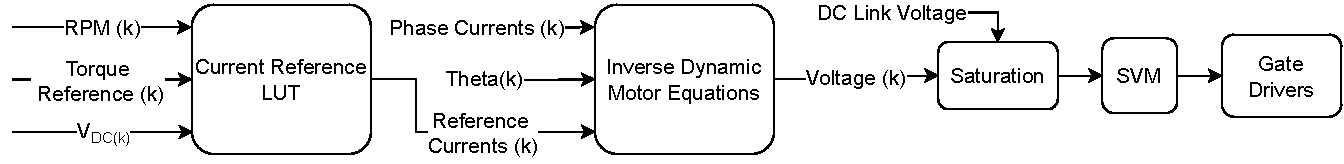
\includegraphics[width=1\textwidth]{Figures/Explicit_CSMPC.pdf}
	\caption[Explicit Continuous Set MPC Diagram.]{Explicit Continuous Set MPC Diagram.}
	\label{fig:explicit_csmpc_diagram}%chktex 24
\end{figure}

This method greatly reduces the time taken to compute the control action, as instead of trying 7 different possible inputs (or more) it just calculates one time the necessary voltage and clamps it to the attainable values. As this control uses a continuous set, those values are then forwarded to a \gls{svm} system to modulate the \gls{pwm} signals. The diagram of this method is shown in \Cref{fig:explicit_csmpc_diagram}.


%%%%%%%%%%%%%%%%%%%%%%%%%%%%%%%%%%%%%%%%%%%%%%%%%%%%%%%%%%%%%%%%%%%%%%%%
%                                                                      %
%     File: Horizon_extension.tex                                      %
%     Tex Master: Thesis.tex                                           %
%                                                                      %
%     Author: Israel Sother                                            %
%     Last modified: 27 May 2024                                       %
%                                                                      %
%%%%%%%%%%%%%%%%%%%%%%%%%%%%%%%%%%%%%%%%%%%%%%%%%%%%%%%%%%%%%%%%%%%%%%%%
\subsubsection{Horizon Extension}
\label{section:Horizon Extension}%chktex 24

A previously overlooked problem is the compensation of the computational time, as the acquisition and control calculations cannot be done instantly their delay needs to be compensated. The strategy adopted here is to use the motor model equations \Cref{eq:motor_backward_euler_matrix} coupled with the previously calculated control action to predict the system state in the next time step, this is called horizon extension. Usually, this is done in a fixed timestep manner, where the predictive controllers instead of picking the control action for $k$ in the timestep $k$, pick the control action for $k+1$ in the timestep $k$, as shown in \Cref{eq:horizon_default} where $x$ represent the currents, $u$ is the voltage vector, $A$, $B$, $C$, and $D$ are the matrices and vectors of the model in \Cref{eq:motor_backward_euler_matrix} and are all dependent on the prediction duration $h = \frac{1}{f_{sw}}$.
\begin{equation}
	x_{k+1} = A^{-1} \left (B x_k + C u_k + D\right )
	\label{eq:horizon_default}
\end{equation}

For this equation to work the system timeline needs to be as in \Cref{fig:horizon_default_timeline}, starting with taking the current and voltage measurements, followed by applying the voltage vectors calculated in $k-1$, then extending the horizon by one timestep, and calculating the voltage vector for the next timestep~\cite{Vazquez:MPC_uses:2014}.

\begin{figure}[!htb]
	\centering
	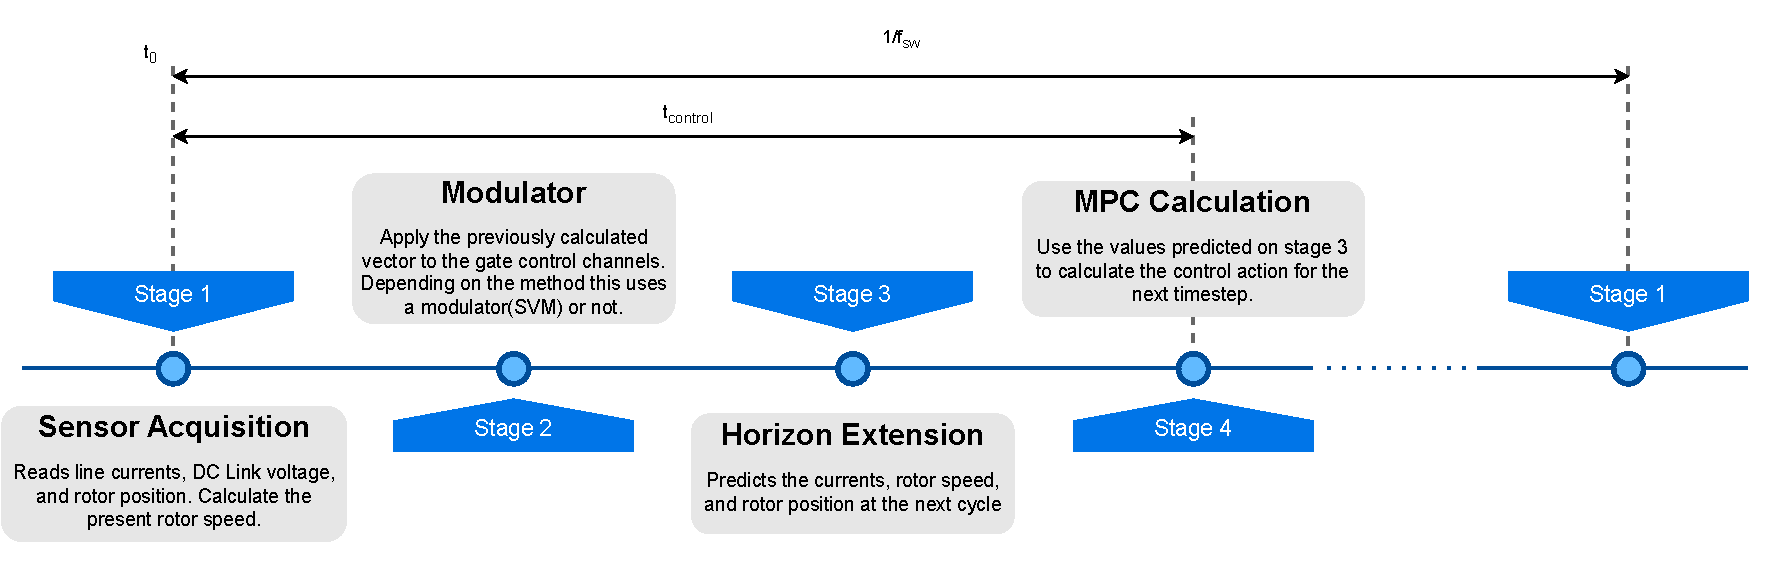
\includegraphics[width=1\textwidth]{Figures/Horizon Extension default Timeline.pdf}
	\caption[Horizon extension by one timestep.]{Horizon extension by one timestep.}
	\label{fig:horizon_default_timeline} %chktex 24
\end{figure}

This can be improved by only extending the horizon by the necessary time to compute the control action, this way the prediction error derived from model mismatch is reduced because the amount of time to predict is smaller. To do that the prediction duration is simply reduced to $h = t_{control}$, while the system timeline is shifted as in \Cref{fig:horizon_extend_timeline}. 


\begin{figure}[!htb]
	\centering
	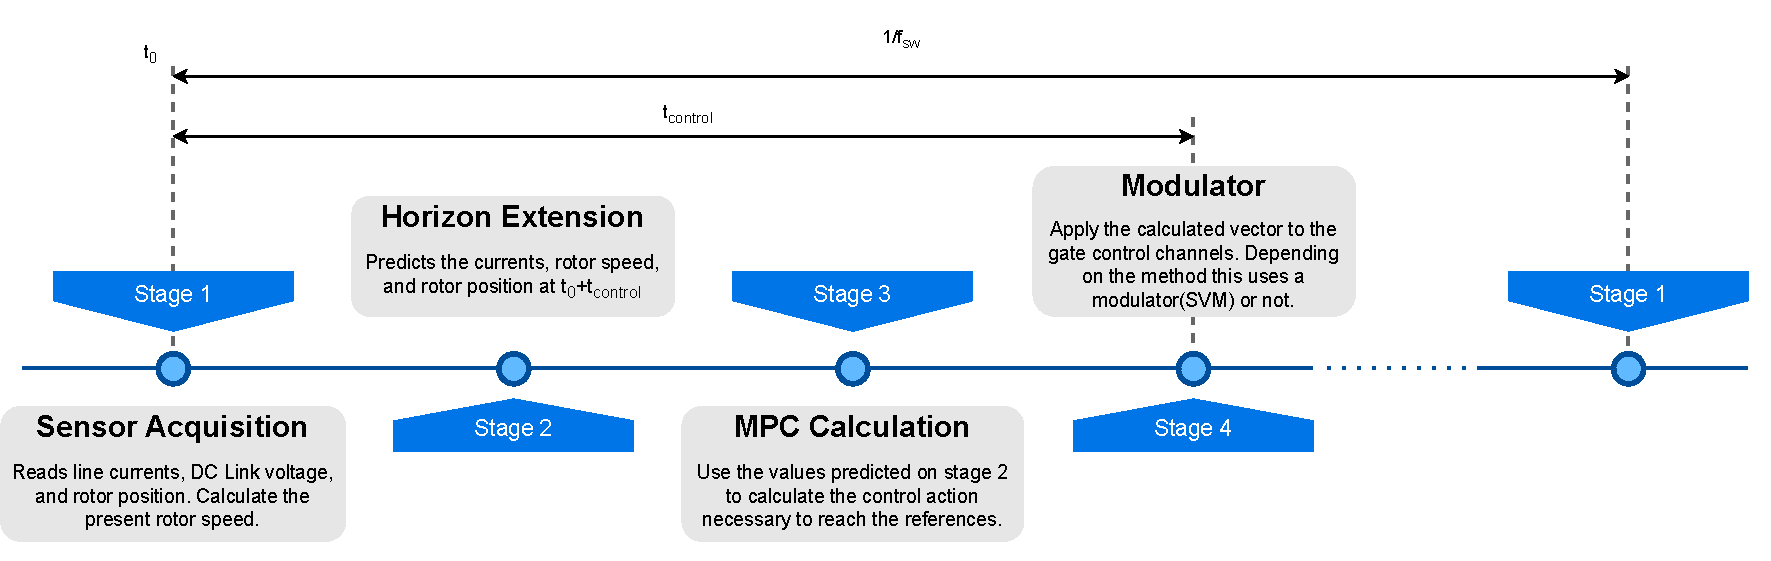
\includegraphics[width=1\textwidth]{Figures/Horizon Extension Timeline.pdf}
	\caption[Horizon Extension by control time.]{Horizon Extension by control time.}
	\label{fig:horizon_extend_timeline} %chktex 24
\end{figure}

The final control cycle starts with sensor acquisition, followed by horizon extension, and lastly the future control action computation. Note that this delay is not a problem with simulation in \textit{Simulink}, as it can instantly do the calculations, but it is good practice to simulate it with the proper delays to increase the similarity between simulation and experimental results.

A comparison of the different horizon extension methods is shown with example values in \Cref{fig:hor_comparison}. Here $\overline{\hat{i}_{dq}}$ represents the norm of the estimated dq current at the end of the horizon extension, $\overline{V_{dq}}$ is the norm of the dq voltage applied by the \gls{svm}, and $\overline{V^*_{dq}}$ is the norm of the computed dq voltage reference. The lines on the top represent the predicted and measured currents, while the lower lines are the voltages. Note that the markers in this figure are placed on the exact time the hardware finishes each computation, thus the delay between measurement, extension, and control calculation. The dashed voltage line represents the moment when the control action reference was computed, so in the regular horizon extension it is ahead of the applied control action as it needs to wait for the next \gls{svm} cycle to be applied. The ultra short horizon technique allows it to be applied as soon as it is computed, resulting in the computed reference and \gls{svm} applied voltages overlapping. Note that the use of a reduced horizon also improves the model mismatch, as the integration error is reduced shown by the reduced lag between the predicted and real currents in \Cref{fig:hor_comparison}.
\begin{figure}[!htb]
	\centering
	\begin{subfigmatrix}{2}
		\subfigure[Default Horizon Extension.]{
			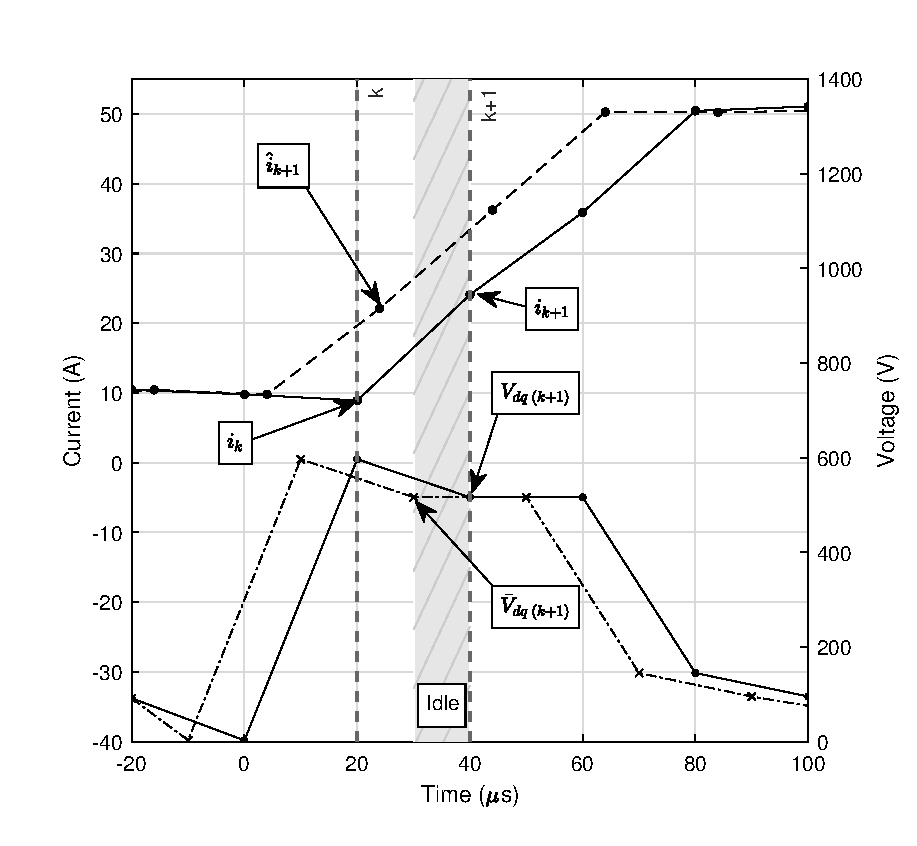
\includegraphics[width=.47\textwidth]{Figures/long_horizon.eps}
			\label{fig:normal_timeline}
		}
		\subfigure[Ultra Short Horizon Extension.]{
			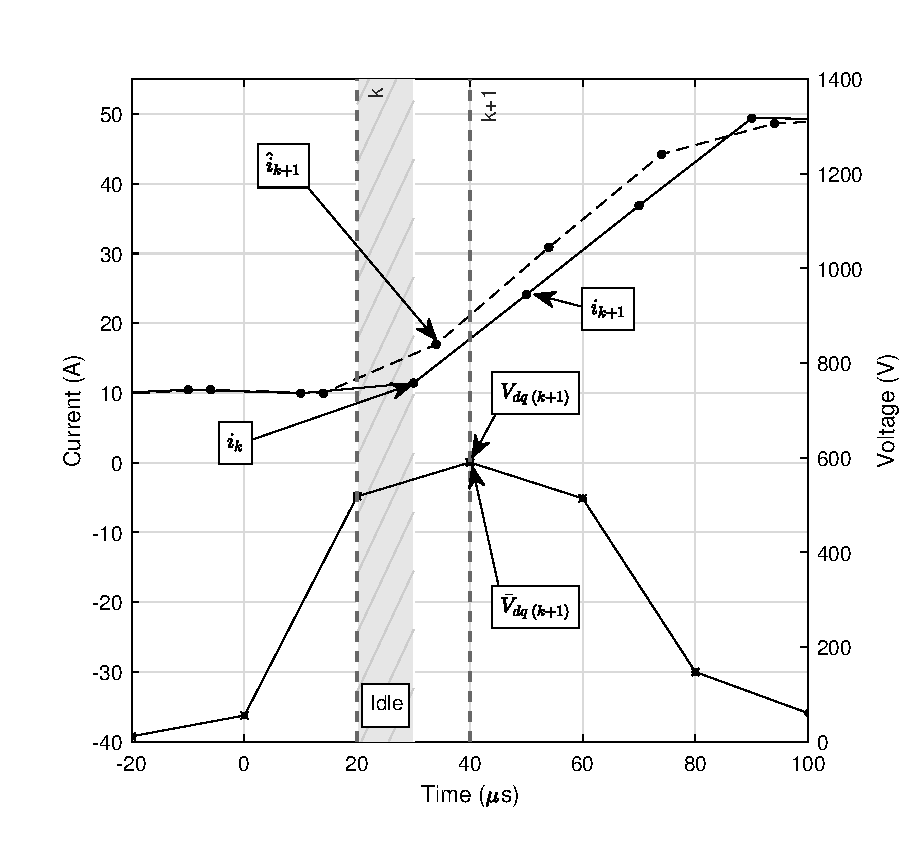
\includegraphics[width=.47\textwidth]{Figures/short_horizon.eps}
			\label{fig:USH_timeline}
		}
	\end{subfigmatrix}
	\caption{Horizon extension comparison, on top the measured and predicted voltages. The bottom lines are the computed control action and the applied control action}
	\label{fig:hor_comparison}
\end{figure}

The combination of explicitly solving the \gls{mpc} model equation with the hybrid horizon timestep approach, where the horizon extension has a shorter timestep than the controllable horizon is called \acrfull{rush}. It has the benefits of being a continuous set model predictive control, thus reducing the ripple, while being computationally efficient, as it is explicitly calculated, and reducing the prediction error due to model mismatch as it uses the reduced horizon extension technique.


\subsubsection{Speed Control}
\label{section:speed_control}%chktex 24

In the current architecture, the car has a slip controller that is responsible for limiting the wheels slip ratio. This controller is based on limiting the maximum (or minimum in the case of braking) speed that a wheel can have. In order to implement this it is necessary to have a rotor speed control. While this could be implemented directly on the \gls{mpc}, the speed dynamics are much slower than the current dynamics, and as such, it is possible to use a simpler control method. The proposed method is a PI controller that receives the rotor speed error and outputs a torque reference. This torque reference is then passed through a saturation which has the limits defined by the throttle and brake pedals, and the resultant torque is used as the input for the \gls{mpc} controllers. The saturation of torque is considered in the integral part of the PI, clamping it if the output is saturated. This structure is shown in \Cref{fig:speed_control_diagram}.

\begin{figure}[!htb]
	\centering
	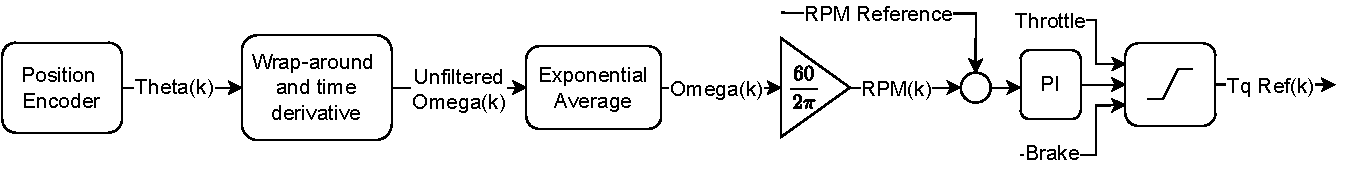
\includegraphics[width=1\textwidth]{Figures/Speed_control.pdf}
	\caption[Speed control diagram.]{Speed control diagram.}
	\label{fig:speed_control_diagram}%chktex 24
\end{figure}

Note that \Cref{fig:speed_control_diagram} also presents a calculation for the rotor speed, this is done by calculating the difference in rotor position between two-time steps and dividing by the sample time. As the rotor position encoder is absolute the position value has a wrap-around point, and thus to calculate the position time derivative an assumption is made that the rotor position does not change more than 180 degrees between two samples. This assumption is valid as the maximum speed of the motor is $20000 rpm$, which translates to $333 Hz$, and the sample time of the encoder is smaller than  $70\mu s$, meaning that the rotor can only move $8.4 \degree$ between samples. This value can increase in the case of a failure in the encoder, but the margin is large enough to accommodate eventual encoder failures. With the rotor position derivative calculated, exponential averaging is applied to smooth the signal and reduce noise, this is done by \Cref{eq:rotor_speed}, where $\alpha$ is the smoothing factor, that defines the weight of the past samples in the current average.

\begin{equation}
	\omega_{(k+1)} = \alpha \omega_{(k)} + (1-\alpha) \frac{\theta_{(k+1)} - \theta_{(k)}}{h}
	\label{eq:rotor_speed}
\end{equation}

A continuous approximation of the exponential moving average can be modeled as a transfer function of a first-order system, with a time constant defined by the smoothing factor $\alpha$, as shown in \Cref{eq:time_constant,eq:exp_moving_average}.


\begin{equation}
	\tau = \frac{-h}{\ln(\alpha)}
	\label{eq:time_constant}
\end{equation}
\begin{equation}
		\frac{\omega}{\omega_{unfiltered}} = \frac{\frac{1}{\tau}}{s+\frac{1}{\tau}}
	\label{eq:exp_moving_average}
\end{equation}

To define the speed controller gains, a simplified motor model was used. As the torque controller is much faster than the speed dynamic, it is assumed to be ideal, without delay. Thus, the speed is only dependent on the motor torque ($T_{e}$), mechanical losses ($T_{loss}$), the external load ($T_{loss}$), and the system inertia ($J$), as shown in \Cref{eq:speed_model}.

\begin{equation}
		\frac{d\omega_{unfiltered}}{dt} = \frac{T_e-T_{load} - T_{loss}}{J}
	\label{eq:speed_model}
\end{equation}

Using the Laplace transform the transfer function is given by \Cref{eq:speed_tf}.

\begin{equation}
		\frac{\omega_{unfiltered}}{T_e} = \frac{1}{J s}-\frac{T_{load} + T_{loss}}{J T_e s}
	\label{eq:speed_tf}
\end{equation}

Assuming the external load, and the mechanical losses as disturbances, the model can be reduced to a first-order system, shown in \Cref{eq:speed_tf_reduced}.

\begin{equation}
		\frac{\omega_{unfiltered}}{T_e} = \frac{1}{J s}
	\label{eq:speed_tf_reduced}
\end{equation}

Combining the motor model with the exponential moving average, a transfer function for the system can be derived, as shown in \Cref{eq:plant_speed_controller}.

\begin{equation}
		H(s) = \frac{\omega}{T_e} = \frac{1}{\tau J s^2+J s}
	\label{eq:plant_speed_controller}
\end{equation}

The controller is defined as a PI controller, thus its transfer function is given by \Cref{eq:controller_speed}.

\begin{equation}
		C(s) = k_p + \frac{k_i}{s}
	\label{eq:controller_speed}
\end{equation}

The closed-loop transfer function from reference speed to filtered speed is then given by \Cref{eq:closed_loop_speed}, while the transfer function from reference speed to actual speed is presented at \Cref{eq:closed_loop_speed_actual}.

\begin{equation}
		\frac{\omega_{measured}}{\omega_{ref}} = \frac{C(s) H(s)}{1+C(s) H(s)} = 
		\frac{k_p s + k_i}{s (J s^2 (\tau + 1) + J s^2)}
	\label{eq:closed_loop_speed}
\end{equation}

\begin{equation}
		\frac{\omega_{real}}{\omega_{ref}} = \frac{(k_p s + k_i)(s\tau + 1)}{J\tau s^3 + J s^2 + k_p s + k_i}
		\label{eq:closed_loop_speed_actual}
\end{equation}

With the transfer function defined, the controller gains can be adjusted to define a critically damped system, with a fast response time. For the testbench used in the experimental validation that has an inertia of approximately $185 g cm^2$, the controller gains were defined as $k_p = 0.035Nm/RPM$ and $k_i = 10^{-9} Nm/RPM$, with the smoothing factor $\alpha = 0.8$. The resulting root locus plot is shown in \Cref{fig:root_locus_speed}, where the poles are located at $-3984.8$, $-3602.0$, and $0$.

\begin{figure}[!htb]
	\centering
	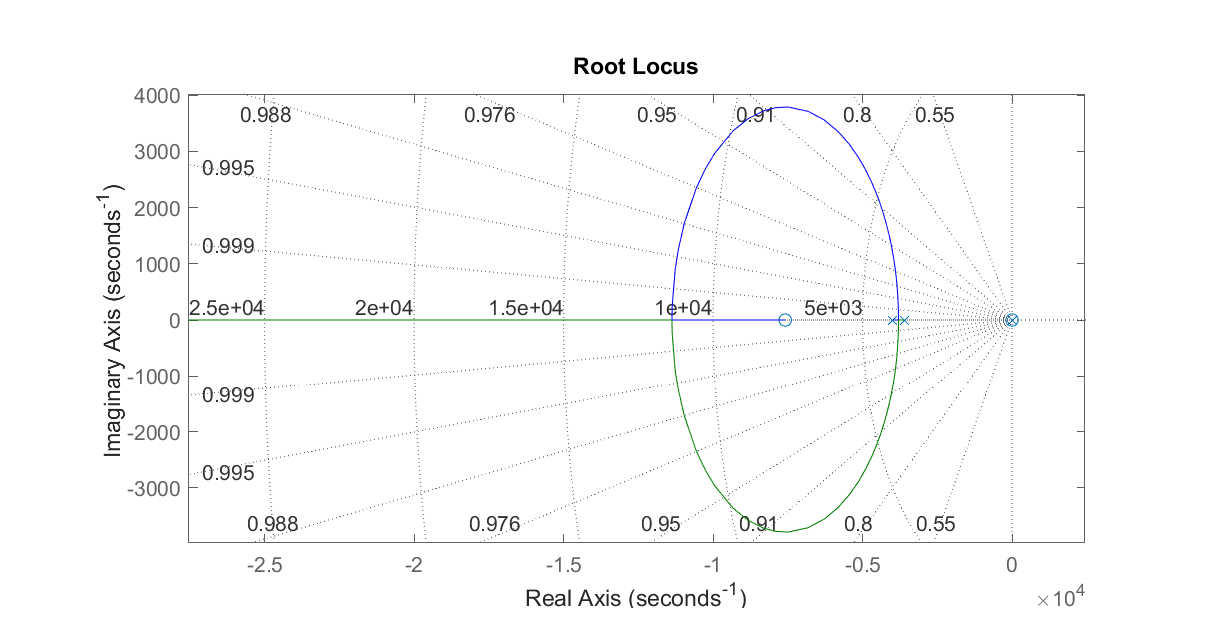
\includegraphics[width=1\textwidth]{Figures/rlocus_speed.eps}
	\caption[Root locus plot for the closed loop system.]{Root locus plot for the closed loop system.}
	\label{fig:root_locus_speed}%chktex 24
\end{figure}